\section{Concept Mapping}
\label{section:concept}

\subsection{Problem Definition}
\emph{Concept mapping} in the context of \emph{GESTALT} is the process of extracting and explicitly encoding the implicit geographic relationships between objects. 
Concept maps are the core of \emph{GESTALT}s geospatial search functionality, supporting two kinds of querying. 
The details of \emph{Location-Centric} and \emph{Object-Centric} pictoral queries are discussed in greater detail in section \ref{section:search}.
Object-Centric queries require a concept map that describes all n-ary object-object relations, where Location-Centric queries only need describe the set of binary object-location relations.
These problems of searching by geographic sets of objects have previously been characterised as graph-matching problems. 
As a graph-matching problem, the difference between a fully connected graph, and a hub-and-spoke graph is significant, particularly as the number of verticies increases. It quickly becomes intractable. \osullikomment{[CITE HERE]}

\osullikomment{Tried to motivate complexity here, but maybe this belongs in search?}

To reduce the complexity, we focus on pruning. 
The first round of pruning occurs when the user selects the \emph{region} that they wish to search. 
\emph{GESTALT} is a last-mile search tool that assumes the user has a general idea of the location (region) that they wish to search. 
The second layer prunes out all locations that do not pass a set-membership test. The arrangement of objects in a location is irrelevant if they don't exist there. 
The third layer occurs during the search of the concept maps, with impossible results being pruned at each step to reduce the total search space to a tractable size. 

\subsubsection{Object-object relations}
The representation of object-object relations as a concept map is grounded in the assumption that the provided query input is a pictoral query. 
When humans descrivbe locations to each other, they frequently draw a map. 
We discuss pictoral querying further in section \ref{section:search}, but intuitively we want to be able to compare a user's sketch map to the real world locations \emph{GESTALT} records. 
Rather than use a fully-connected graph, we encode both the locations, and later, the pictoral query inputs as matricies with zeros representing unallocated space and the names of objects. 
The matricies are $NxN$, where $N$ is the number of objects at a location. 
Using algorithm \ref{alg:geoToGrid}, we assign each object in a given location to a position $(i,j)$ in the Matrix where $i$ is its order of appearance from north to south and $j$ is the same object's order of appearance from west to east. 
The result is a matrix in which each row and column has only a single object. 
Where ties are experienced in the real world (due to a lack of GPS precision, or very close position) they are broken lexiographically in the object-object concept map instantiation.
The process of creating and querying a concept map is shown in Figure \ref{figure:ConceptMap}.

\paragraph{Query Input}

\begin{figure*}[h]
    \centering
    
    \begin{subfigure}[t]{.3\textwidth}
        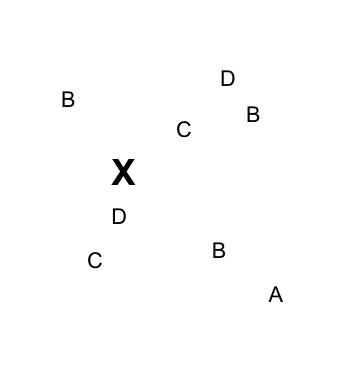
\includegraphics[width=\textwidth]{CM-ExampleLocation.png}
        \caption{\small A candidate location X has named objects A-D with the spatial layout depicted above.} % The increasing focus on questions targeting secret information drives down false positives (paranoia) across models but dramatically increases false negatives (leakage).
        \label{fig:CM-Example}
    \end{subfigure}
    \hfill
    \begin{subfigure}[t]{.3\textwidth}
        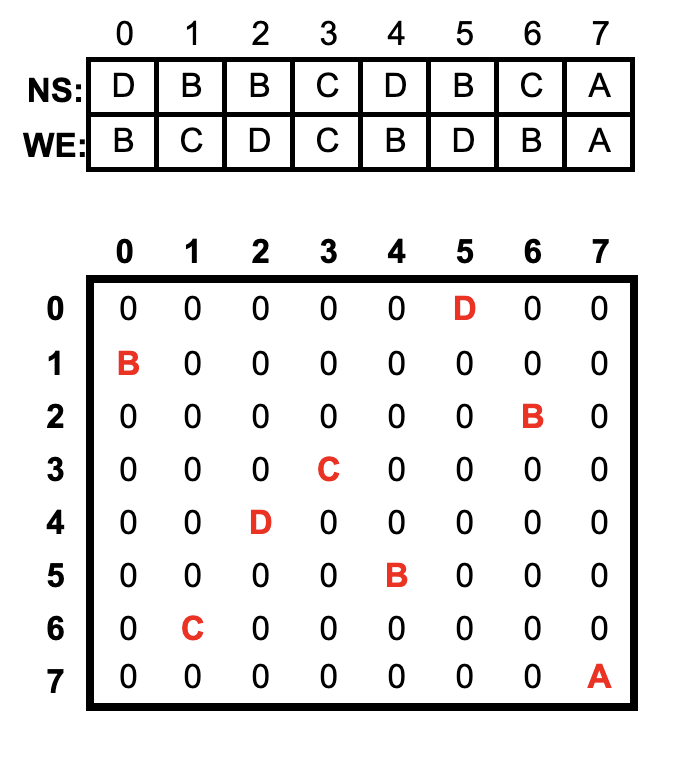
\includegraphics[width=\textwidth]{CM-OO-Setup.png}
        \caption{\small During pre-processing, the objects associated with location X are ordered North to South (NS) and West to East (WE) and mapped into a matrix with corresponding indices.} % Increasing the number of secrets kept drives a small but consistent increase in false positives (paranoia).
        \label{fig:CM-OO-Setup}
    \end{subfigure}
    \hfill
        \begin{subfigure}[t]{.3\textwidth}
        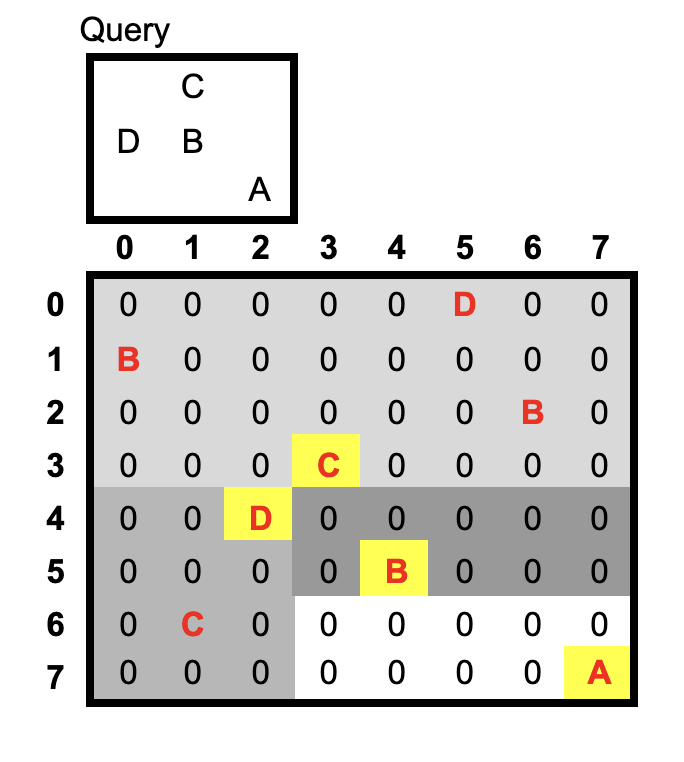
\includegraphics[width=\textwidth]{CM-OO-Query1.png}
        \caption{\small Searching recursively prunes for ANY match. Each recursion is a darker shade, with unpruned area in white. Objects highlighted in yellow are found to match the query configuration; candidate location X is a match for the query.}% Increasing the amount of secret context available to models improves performance, but we still see some generalization with only a quarter of the secret context provided to the system.
        \label{fig:CM-OO-Query}
    \hfill
    \end{subfigure}
    \caption{\textbf{Generate and Query an Object-Object Concept Map.}}\label{figure:ConceptMap} 
\end{figure*}
- algorithm for parsing from grid, etc.


\paragraph{Solution}

\begin{algorithm}
    \caption{Recursive Grid Search}\label{alg:gridSearch}
    \begin{algorithmic}
        \State{\textit{\textbf{M} A ConceptMap Matrix with objects or 0s; [0,0] is NW most point}}
        \State{\textit{\textbf{L} A NW to SE ordered list of objects to search for}}
        \State{\textit{\textbf{D} The direction of Pruning, 'northToSouth' or 'westToEast'}}
        \State{- - - - -}
        \Procedure{recursiveGridSearch}{$M$,$L$,$D$} %\Comment{$M$ a matrix of a Loc's objects, $L$ an ordered list of objects to search for, $D$ is the pruning direction}

            \If{$L$ has only 1 item}\Comment{Base Case}
                \If{pop($L$) in $M$}
                    \State{\textbf{return} $True$}              
                \Else
                    \State{\textbf{return} $False$}
                \EndIf            
            \EndIf


            \If{$D$ is $northToSouth$}
                \State{$NorthernObject$ = pop($L$)}                
                \If{$NorthernObject$ not in $M$}
                    \State{\textbf{return} $False$}               
                \EndIf

                \State{$M$ = Prune all objects north of $NorthernObject$}
                \State{\textbf{return recursiveGridSearch}($M$,$L$,$westToEast$)}
           
            \EndIf

            \If{$D$ is $eastToWest$}
                \State{$WesternObject$ = pop($L$)}
                
                \If{$WesternObject$ not in $M$}
                    \State{\textbf{return} $False$}
                \EndIf

                \State{$M$ = Prune all objects west of $WesternObject$}
                \State{\textbf{return recursiveGridSearch}($M$,$L$,$northToSouth$)}
            \EndIf

        \EndProcedure

    \end{algorithmic}

\end{algorithm}



- recursive algorithm for finding any match
- complexity analysis

\paragraph{Experimental Results?}
- on ground truth queries? report number of locations pruned? timings?




\subsubsection{Object-Location relations}
- description...........
- diagram showing input and expected output.........

\begin{figure*}[h]
    \centering
    
    \begin{subfigure}[t]{.3\textwidth}
        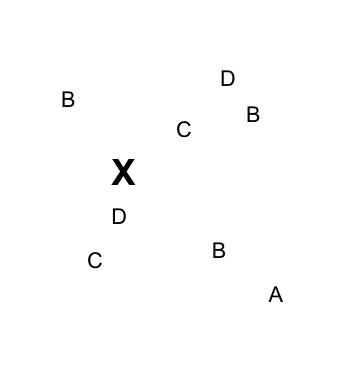
\includegraphics[width=\textwidth]{CM-ExampleLocation.png}
        \caption{\small A candidate location X has named objects A-D with the spatial layout depicted above.} 
        \label{fig:CM-LO-Example}
    \end{subfigure}
    \hfill
    \begin{subfigure}[t]{.3\textwidth}
        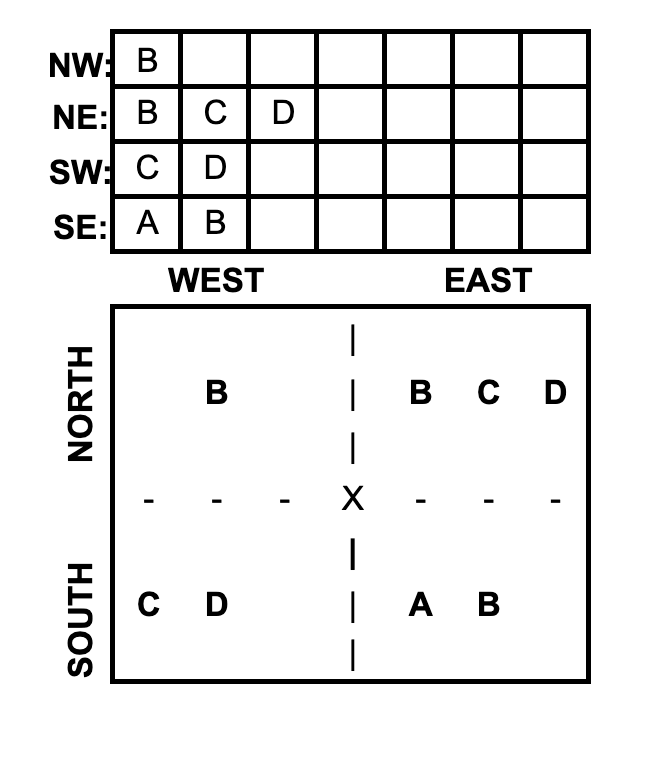
\includegraphics[width=\textwidth]{CM-LO-Setup.png}
        \caption{\small The objects are binned into spatial quadrants based on their relative position to the location centroid, X.} 
        \label{fig:CM-LO-Setup}
    \end{subfigure}
    \hfill
        \begin{subfigure}[t]{.3\textwidth}
        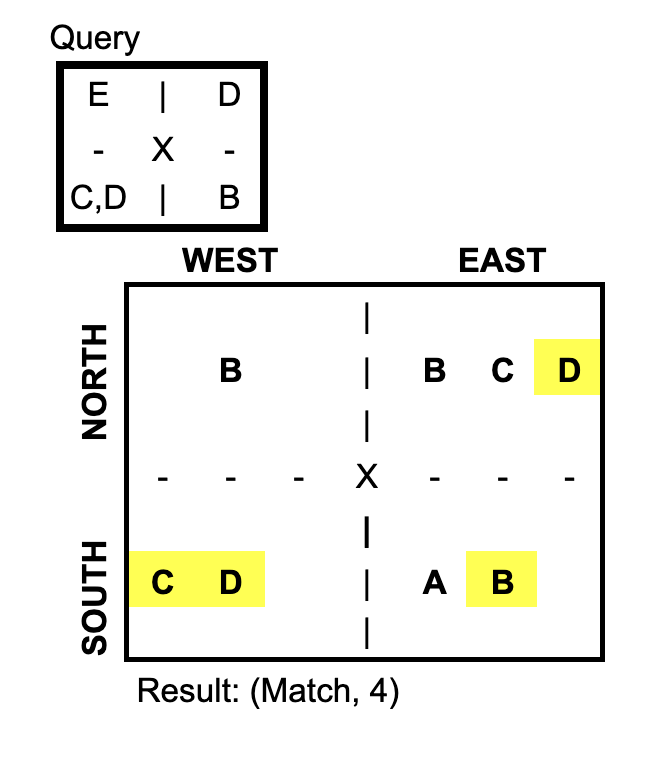
\includegraphics[width=\textwidth]{CM-LO-Query1.png}
        \caption{\small Searching counts the number of query terms that correspond to a location's quadrants and returns the count, allowing multiple candiate solutions to be ranked by closeness of match.}
        \label{fig:CM-LO-Query}
    \hfill
    \end{subfigure}
    \caption{\textbf{Generate and Query an Location-Object Concept Map.}}\label{figure:ConceptMap-LO} 
\end{figure*}




\paragraph{Query Input}
- algorithm for parsing from grid, etc.

\paragraph{Solution}
- recursive algorithm for finding any match
- complexity analysis

\paragraph{Experimental Results?}
- on ground truth queries? report number of locations pruned? timings?


%Concept mapping has been partially implemented in Python leveraging the \textit{Scipy} library\footnote{\href{https://pypi.org/project/scipy/}{SciPy PyPI Repo}}. Two different approaches have been trialed. 
%The first is simple dynamic arithmetic on the coordinates stored in a Pandas data frame. If one set of coordinates is above, below, left or right of another, it is north, south, east or west, respectively. 
%While these calculations are in constant time for straightforward comparisons of known objects (e.g. "is the pond west of the bridge"), the time complexity rapidly increases as soon as aggregations are employed. 
%Queries of "Give me everything west of the duck pond" would execute in $O(N)$ time as each element has to be examined. Worst-case queries would run in $O(N\sup{2})$ time, where every object is checked for its position relative to every other object. 

%The second (better) approach (only partially implemented) instantiates the objects within a location into a KD-Tree. 
%Assuming that the object centroid is the root, we can quickly complete queries like "Give me everything west of the duck pond" by leveraging the structure of the subtrees to return the requested set. 
%Similarly, getting the relative positions of two objects searches for a common ancestor. It uses the path between the children and their ancestor node to infer their spatial relation to each other.

%A third approach, designed to leverage the \textit{Neo4J Python Library}\footnote{\href{https://pypi.org/project/neo4j/}{Neo4J PyPI Repo}} to connect to a \textit{Neo4J Graph Database}\footnote{\href{https://neo4j.com/}{Neo4J Website}} but not implemented frames concept mapping as a graph traversal problem. 
%In this formulation, each object is a node on a graph. Weighted, labeled edges exist between each node within a given proximity threshold to the node. 
%The edge labels describe the neighboring node's cardinal direction and the distance weights. 
%After constructing the object graph, queries for 'give me everything west of the duck pond' would freely explore nodes connected by west, north and south edges. 
%It can only traverse along an east edge so long as the total cost of traveling east would be less than the cumulative value of the 'west' travel up to this point. 

%%Overall, concept mapping aims to enable geographic search over objects by explicitly representing their geospatial relationships to each other. 
%The author implemented a very basic approach using coordinate arithmetic was quickly determined to be infeasible for the extensive data sets that \textit{GESTALT} anticipates processing. 
%KD-Trees for the objects in each location have been implemented, as have the KD-Trees for the locations themselves. 
%This conceptual KD-Tree of KD-Trees approach performs a natural aggregation function which, provided that regions are created consistently, will allow for relative spatial queries at different levels of granularity. 
%Empirical evaluation of the performance of the arithmetic, KD-Tree and Graph-based approaches is yet to be completed. 



%%%%%%%%%%%%%%%NSCH clean up, incorporate, and delete the text below this point
Concept mapping is the process of determining the geospatial relations between objects. Much information is implicit in the relative positioning of objects within a location. For \textit{GESTALT}, there are three types of relations. 
The first is \textit{Static Cardinal Relations} which encodes whether an object is North, South, East or West of a location. Static Cardinal Relations support simple queries where the user knows that a location has a lake on its western side. 
The second is \textit{Dynamic Cardinal Relations} which determines whether an object is North, South, East or West of another object within a location. These queries support cases where a searcher might remember standing at a lake northeast of a location and that there was a swingset to the immediate west of them but still in the northeast of the location overall. 
The third are \textit{Positional Relations} which are applied to the two other types to enable reasoning about objects that are left, right, up, down, beside, behind etc., other objects. 
Positional relation use will be extensive because few humans think in cardinal directions, and most spatial reasoning is conducted from the person's perspective. 
Positional Relations enable users to query for locations where there is a letterbox on the left of the driveway as you enter the driveway while the house is in front of you. 

Concept mapping needs to be unsupervised and support aggregation. Tracking every object's relative location to every other object quickly becomes intractable, so mechanisms to aggregate depending on the level of granularity need to be applied. 
Accordingly, the underlying data structure must support aggregation and relative position querying. 